\chapter{Lesson-2 What is Machine Learning?}
\section{What is machine learning?}
To make a really easy definition let's think about this: in the world exist humans and computers, we already know that humans get knowledge from past experiences in the other hand computers need to be programmed to know what to do so we need to made the question: ¿Computers can also get knowledge from past experiences too? and this is the answer that machine learning can give us. Obviously for a computer "past experiences" are just data, so we go to learn how to use this data to develop machine learning.

\section{Decision trees}
Let's start with a simple example, imagine that we need to recommend applications from the google play store to each user.

\begin{longtable}[c]{@{}lll@{}}
    \rowcolor[HTML]{010066}
    {\color[HTML]{FFFFFF} \textbf{Gender}} & {\color[HTML]{FFFFFF} \textbf{Age}} & {\color[HTML]{FFFFFF} \textbf{App}} \\*
    \endfirsthead
    %
    \endhead
    %
    \rowcolor[HTML]{FFFFFF}
    F                                      & 15                                  & {\color[HTML]{333333} Pokemon go}   \\
    F                                      & 25                                  & Whatsapp                            \\
    M                                      & 32                                  & Snap chat                           \\
    F                                      & 40                                  & Whatsapp                            \\
    M                                      & 12                                  & Pokemon go                          \\
    M                                      & 14                                  & Pokemon go                         
\end{longtable}

Consider the table above and answer \textsf{Between \textbf{gender} and \textbf{age}, which one seems more decisive for predicting what app the users will download?} the answer is very simple, is the age, as we can see we get more information about the preferences between all the applications that we have in the table. But let's do this analysis step by step, let's split the table first using the gender:

\begin{longtable}[c]{lll}
    \rowcolor[HTML]{010066} 
    {\color[HTML]{FFFFFF} \textbf{Gender}} & {\color[HTML]{FFFFFF} \textbf{Age}} & {\color[HTML]{FFFFFF} \textbf{App}} \\
    \endfirsthead
    %
    \endhead
    %
    \rowcolor[HTML]{FFCCC9} 
    F                                      & 15                                  & {\color[HTML]{333333} Pokemon go}   \\
    \rowcolor[HTML]{FFCCC9} 
    F                                      & 25                                  & Whatsapp                            \\
    \rowcolor[HTML]{CBCEFB} 
    M                                      & 32                                  & Snap chat                           \\
    \rowcolor[HTML]{FFCCC9} 
    F                                      & 40                                  & Whatsapp                            \\
    \rowcolor[HTML]{CBCEFB} 
    M                                      & 12                                  & Pokemon go                          \\
    \rowcolor[HTML]{CBCEFB} 
    M                                      & 14                                  & Pokemon go                         
\end{longtable}

As we can see female users have downloaded Pokemon go and WhatsApp in the other hand male users have downloaded Snap Chat and Pokemon Go. So we can get good sets using the gender. \hfill \break

Now we go to make the same analysis but now we go to use the age, let's consider the users that have 20 or less age as one set and more of 20 as the other one.

\begin{longtable}[c]{lll}
    \rowcolor[HTML]{010066} 
    {\color[HTML]{FFFFFF} \textbf{Gender}} & {\color[HTML]{FFFFFF} \textbf{Age}} & {\color[HTML]{FFFFFF} \textbf{App}} \\
    \endfirsthead
    %
    \endhead
    %
    \rowcolor[HTML]{FFCCC9} 
    F                                      & 15                                  & {\color[HTML]{333333} Pokemon go}   \\
    \rowcolor[HTML]{CBCEFB} 
    F                                      & 25                                  & Whatsapp                            \\
    \rowcolor[HTML]{CBCEFB} 
    M                                      & 32                                  & Snap chat                           \\
    \rowcolor[HTML]{CBCEFB} 
    F                                      & 40                                  & Whatsapp                            \\
    \rowcolor[HTML]{FFCCC9} 
    M                                      & 12                                  & Pokemon go                          \\
    \rowcolor[HTML]{FFCCC9} 
    M                                      & 14                                  & Pokemon go                         
\end{longtable}

As we can see we get better results using the age. For example the people under 20 years old use to download pokemon go, does not matter if there are male or female. But it is a little bit different with whatsapp and snap chat, in this case if the user is female the application that they used to use is whatsapp otherwise is snap chat. We can see this using the next diagram.

\diagramtikz{
    \begin{center}
        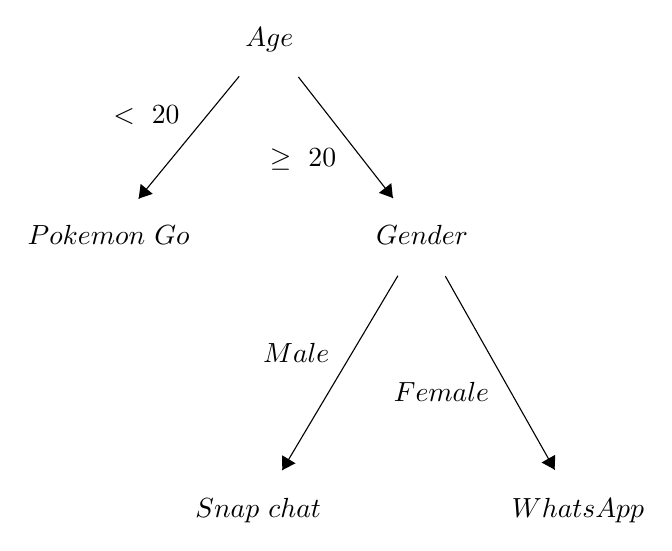
\begin{tikzpicture}[scale=0.2]
        \tikzstyle{every node}+=[inner sep=0pt]
        \draw (39.9,-7.1) node {$Age$};
        \draw (29.7,-19.5) node {$Pokemon\mbox{ }Go$};
        \draw (49.6,-19.5) node {$Gender$};
        \draw (39.2,-37) node {$Snap\mbox{ }chat$};
        \draw (59.5,-37) node {$WhatsApp$};
        \draw [black] (37.99,-9.42) -- (31.61,-17.18);
        \fill [black] (31.61,-17.18) -- (32.5,-16.88) -- (31.73,-16.25);
        \draw (34.24,-11.87) node [left] {$<\mbox{ }20$};
        \draw [black] (41.75,-9.46) -- (47.75,-17.14);
        \fill [black] (47.75,-17.14) -- (47.65,-16.2) -- (46.86,-16.82);
        \draw (44.18,-14.71) node [left] {$\geq\mbox{ }20$};
        \draw [black] (48.07,-22.08) -- (40.73,-34.42);
        \fill [black] (40.73,-34.42) -- (41.57,-33.99) -- (40.71,-33.48);
        \draw (43.75,-26.99) node [left] {$Male$};
        \draw [black] (51.08,-22.11) -- (58.02,-34.39);
        \fill [black] (58.02,-34.39) -- (58.06,-33.45) -- (57.19,-33.94);
        \draw (53.89,-29.47) node [left] {$Female$};
        \end{tikzpicture}
    \end{center}
}{Decision tree}{Diagram:01}

\section{Naive bayes}
